\documentclass{article}
\usepackage[T1]{fontenc}
\usepackage{amssymb}
\usepackage{listings}
\usepackage[utf8x]{inputenc}
\usepackage{amsmath,amssymb}
\usepackage{pdfpages}
\usepackage[russian,english]{babel}
\lstset{
    language=Octave,
    frame=single,
    inputencoding=utf8x,
    extendedchars=\true,
    texcl=\false,
    breaklines=true,
    breakatwhitespace=true,
    commentstyle={}
}
\usepackage[a4paper,top=1cm,bottom=2cm,left=1.5cm,right=1cm,marginparwidth=1.75cm]{geometry}

\makeatletter
\def\@seccntformat#1{
  \expandafter\ifx\csname c@#1\endcsname\c@section\else
  \csname the#1\endcsname\quad
  \fi}
\makeatother

\begin{document}

\selectlanguage{russian}
\title{Лабораторная работа 4, ТВМС}
\author{
	Бочарников Андрей, M3238\\
	Ковешников Глеб, M3238\\
	Шишкин Алексей, M3238
}
\maketitle

\begin{quote}
\selectlanguage{russian}
\section{Формулировка}
	Для случайной величины, распределенной по нормальному закону с параметрами ($a$,$\sigma^2$), выполнить следующие действия:\\\\
	1. Задать параметры распределения $X \thicksim N(a, \sigma^2)$.\\
	2. Построить выборку генеральной совокупности $X$.\\
	3. Построить график гистограммы.\\
	4. Проверить гипотезу о виде распределения по критерию хи-квадрат.\\
	Аналогично для $X \thicksim U(a, b)$ - равномерно распределенной на $[a, b]$ случайной величины.
\section{Входные данные}
        \begin{itemize}
            \item Размер выборки для построения гистограммы: $n = 10^6$
	    \item Размер выборки для проверки критерия $\chi^2$: $n = 10^4$
            \item Параметры нормального распределения: $\sigma = 1, \mu = 1$
	    \item Параметры равномерного распределения: $a = 20, b = 80$
            \item $\alpha = 0.05$
	    \item Количество тестов -- $10^3$
        \end{itemize}
\section{Программа 1}
	Нормальное распределение. График гистограммы - график 1 в приложении после вывода. \\
	В первой части программы строится гистрограмма с использованием функции hist и выводится на экран вместе с графиком функции распределения. \\
	Во второй части производится три запуска тестов на проверку гипотез: \\
	1. Выборка генерируется с помощью нормального распределения; нижняя граница на количество элементов попавших в интервал отстутствует; проверяется гипотеза о нормальном распределении; оценивается вероятность ошибки первого рода. \\
	2. Выборка генерируется с помощью нормального распределения; соседние интервалы объединяются, чтобы количество элементов попавших на каждый интервал было не меньше 6; проверяется гипотеза о нормальном распределении; оценивается вероятность ошибки первого рода. \\
	3. Выборка генерируется с помощью нормального распределения; нижняя граница на количество элементов попавших в интервал отстутствует; проверяется гипотеза о равномерном распределении; оценивается вероятность ошибки второго рода. \\
\subsection{Исходный код}
	\lstinputlisting{task1.m}
\subsection{Выходные данные}
	Размер выборки $= 1000000$ \\
	Выбранная длина интервалов $= 0.100212$ \\
	Количество интервалов $= 100$ \\

	Нормальное распределение проходит проверку гипотезы о нормальном распределении \\
	Для $\alpha = 0.05$, вероятность ошибки первого рода получается $0.328$ \\

	Нормальное распределение проходит проверку гипотезы о нормальном распределении \\
	Данные сгруппированы, чтобы выполнялось $n_j >= 6$ \\
	Для $\alpha = 0.05$, вероятность ошибки первого рода получается $0.064$ \\

	Нормальное распределение проходит проверку гипотезы о нормальном распределении \\
	Выборочное среднее и выборочная дисперсия изменены на $0.005$ \\
	Для $\alpha = 0.05$, вероятность ошибки второго рода получается $0.06$ \\

	Нормальное распределение проходит проверку гипотезы о нормальном распределении \\
	Выборочное среднее и выборочная дисперсия изменены на $0.01$ \\
	Для $\alpha = 0.05$, вероятность ошибки второго рода получается 0.05 \\

	Нормальное распределение проходит проверку гипотезы о нормальном распределении \\
	Выборочное среднее и выборочная дисперсия изменены на $0.025$ \\
	Для $\alpha = 0.05$, вероятность ошибки второго рода получается $0.245$ \\

\section{Программа 2}
	Равномерное распределение. График гистограммы - график 2 после вывода. \\
	В первой части программы строится гистрограмма с использованием функции hist и выводится на экран вместе с графиком функции распределения. \\
	Во второй части производится два запуска тестов на проверку гипотез: \\
	1. Выборка генерируется с помощью равномерного распределения; нижняя граница на количество элементов попавших в интервал отстутствует; проверяется гипотеза о равномерном распределении; оценивается вероятность ошибки первого рода. \\
	2. Выборка генерируется с помощью равномерного распределения; нижняя граница на количество элементов попавших в интервал отстутствует; проверяется гипотеза о нормальном распределении; оценивается вероятность ошибки второго рода. \\
\subsection{Исходный код}
	\lstinputlisting{task2.m}
\subsection{Выходные данные}
	Размер выборки $= 1000000$ \\
	Выбранная длина интервалов $= 0.599997$ \\
	Количество интервалов $= 100$ \\

	Равномерное распределение проходит проверку гипотезы о равномерном распределении \\
	Для $\alpha = 0.05$, вероятность ошибки первого рода получается $0.057$ \\

	Равномерное распределение проходит проверку гипотезы о равномерном распределении \\ 
	Левая и правая граница изменены на $0.25$ \\
	Для $\alpha = 0.05$, вероятность ошибки второго рода получается $0.088$ \\

	Равномерное распределение проходит проверку гипотезы о равномерном распределении \\
	Левая и правая граница изменены на $0.75$ \\
	Для $\alpha = 0.05$, вероятность ошибки второго рода получается $0.163$ \\

	Равномерное распределение проходит проверку гипотезы о равномерном распределении \\
	Левая и правая граница изменены на $1.5$ \\
	Для $\alpha = 0.05$, вероятность ошибки второго рода получается $0.667$ \\

\section{Вывод}
	1. Как видно по рисунку, график гистограммы хорошо приближает график плотности распределения. \\ \\
        2. Как и нужно, вероятность ошибки первого рода теста по критерию хи-квадрат для $\alpha = 0.05$, сходится к $0.05$. Вероятность ошибки второго рода для испорченной выборки сходится к $0$.
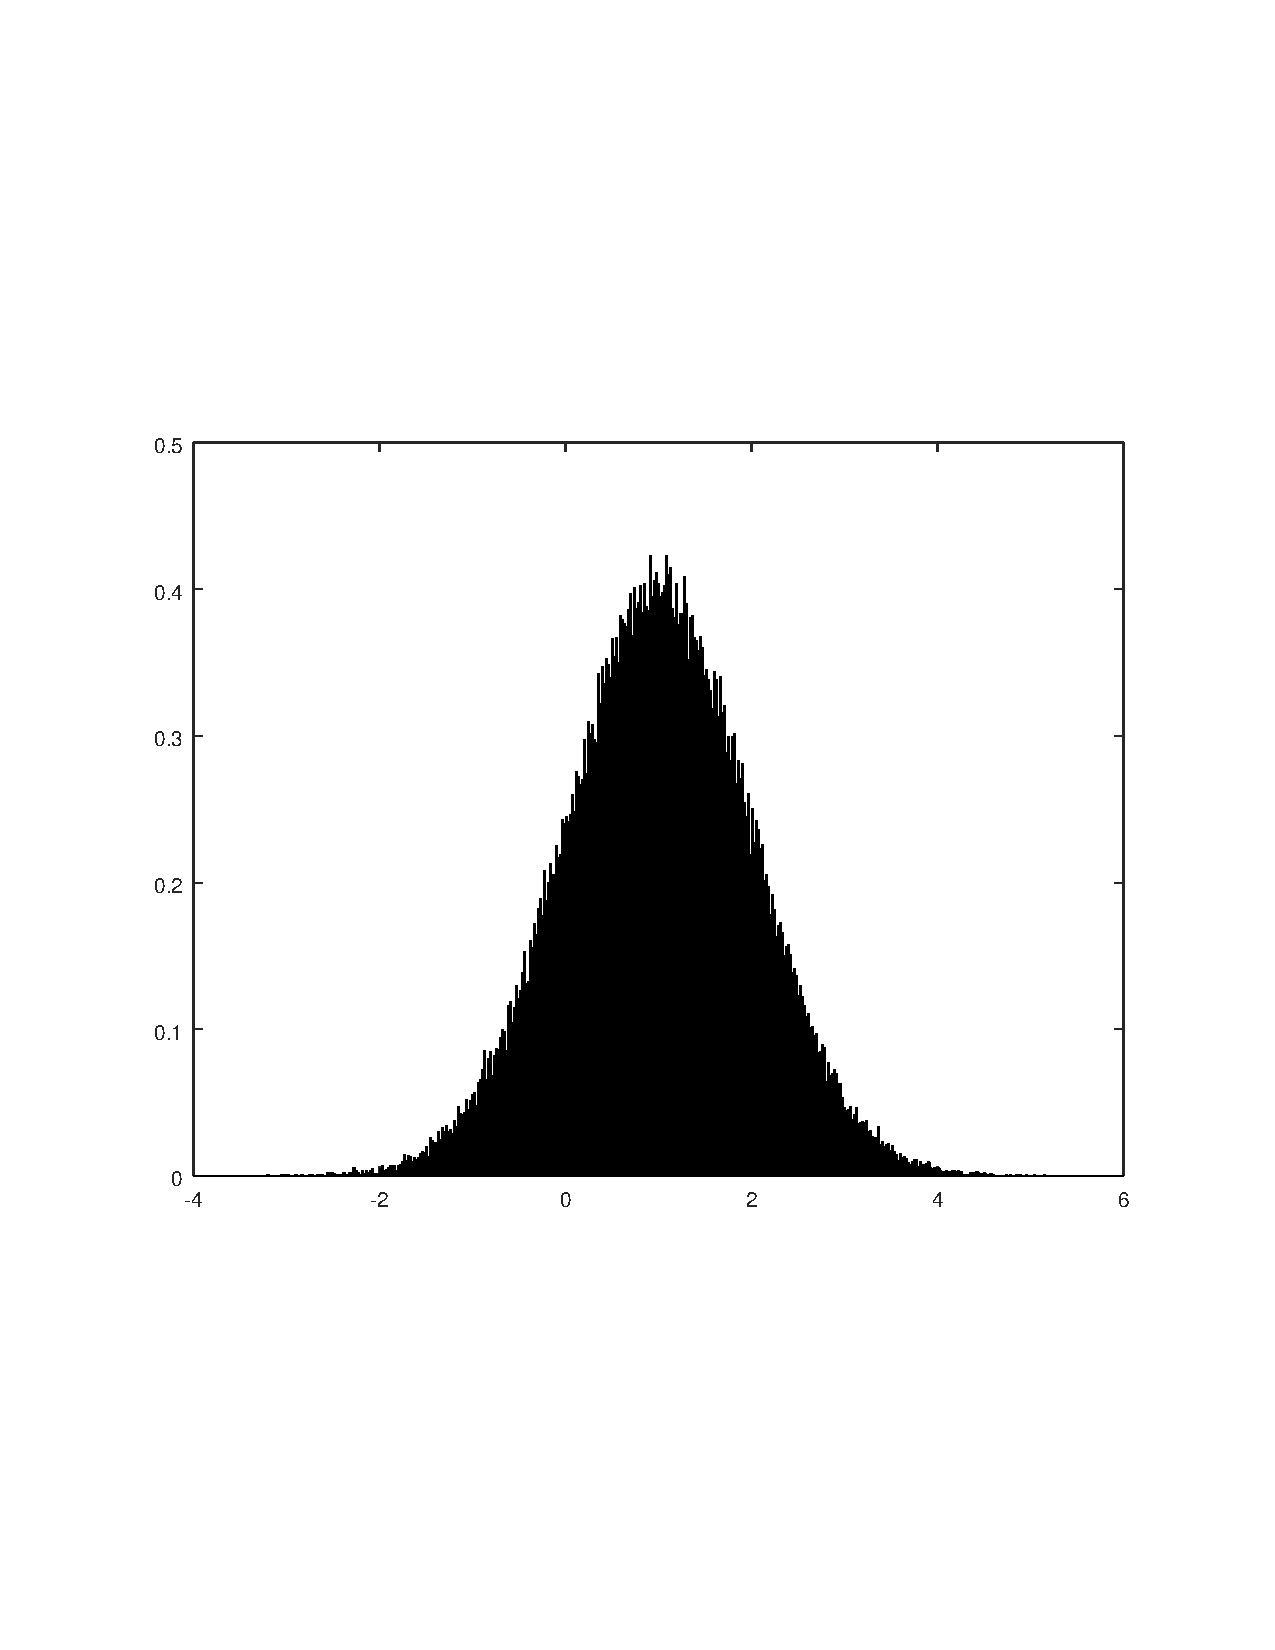
\includepdf[width=\textwidth]{normcdf.pdf}
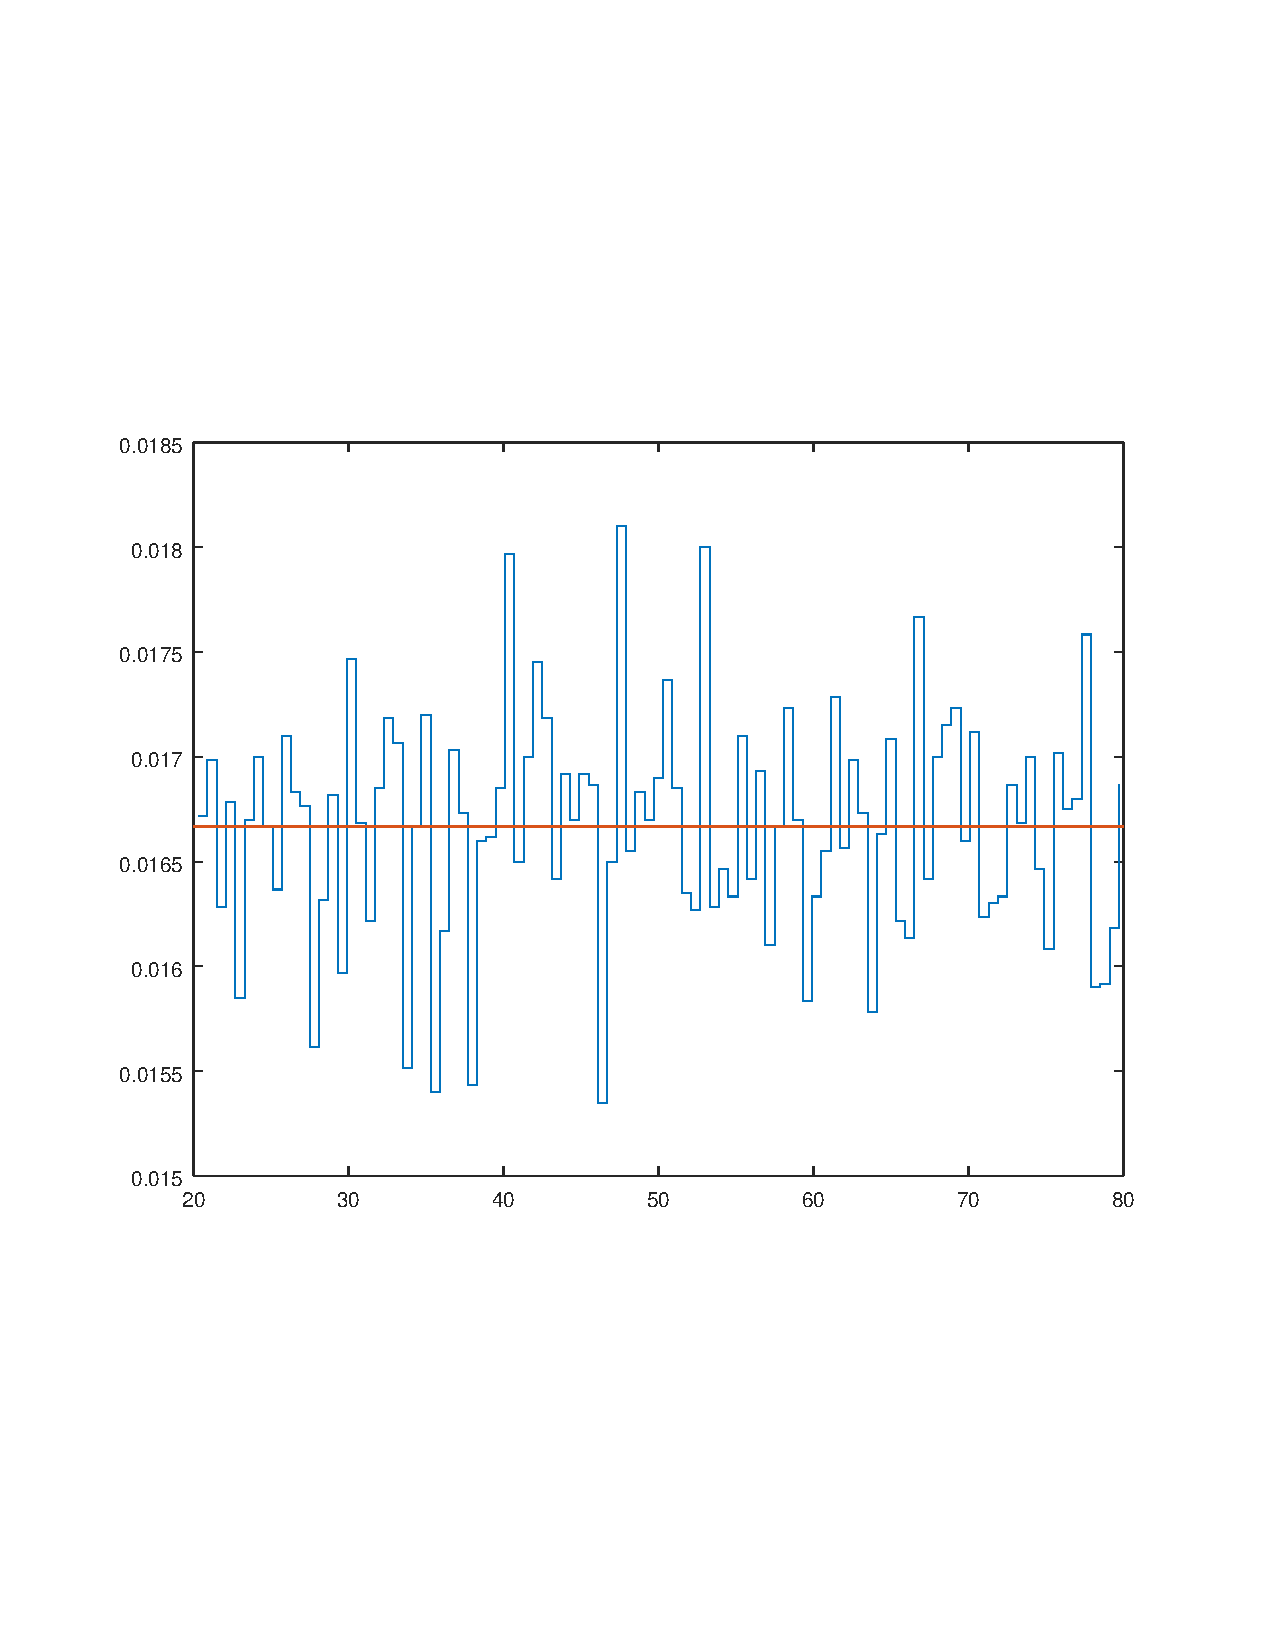
\includepdf[width=\textwidth]{unicdf.pdf}
\end{quote}
\end{document}
